% Set chapter counter to 0 and reset section counter for acknowledgments
\setcounter{chapter}{0}
\setcounter{section}{0}

% Add acknowledgments to table of contents
\addcontentsline{toc}{chapter}{Acknowledgments}

% Set up page style for acknowledgments
\pagestyle{fancy}
\fancyhf{} % Clear all header and footer fields
\fancyhead[L]{\footnotesize\textit{Ars Post Faber: Digital fabrication democratization through embodied knowledge preservation}}
\fancyfoot[C]{\thepage} % Page number in footer center
\renewcommand{\headrulewidth}{0pt}
\renewcommand{\footrulewidth}{0pt}

% Custom acknowledgments title to match chapter formatting
\noindent
{\Large\textbf{Acknowledgments}}
\vspace{0.3cm}
\hrule
\vspace{0.8cm}

% Set no paragraph indentation
\setlength{\parindent}{0pt}

I extend my deepest gratitude to my thesis advisors Jessica Carmen Guy, Roger Guilemany, and Alejandra Tothill, whose feedback, insights, and support helped shape this work.

\subsection{About transparency}

In the interest of transparency and following principles of responsible AI usage in academic research, I acknowledge the use of artificial intelligence tools throughout various phases of this thesis development. This usage is documented according to the Cognitive Contribution License (CCL) framework developed by Santi Fuentemilla at Fab Lab Barcelona.

\begin{figure}[H]
\centering
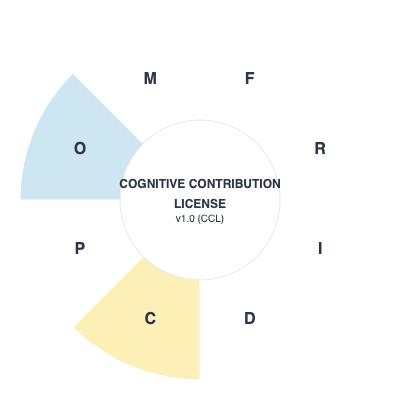
\includegraphics[width=1\textwidth]{figures/acknowledgements/ccl-badge.png}
\caption{Cognitive Contribution Lable (CCL). Source: \citet{santifu_ccl_2024}}
\label{fig:ccl}
\end{figure}


\textbf{CCL Summary:} "Ars Post Faber" by Jorge Muñoz Zanón CCL C2 O1v1.0 — AI acted as Co-Creator in Coding, AI contributed as Drafting Assistant in Documentation. All other phases were fully human-led.

\vspace{0.5cm}

Specifically, artificial intelligence systems contributed to this research in the following capacities:

\vspace{0.5cm}

\textbf{Coding:} AI systems served as co-creators in software development, particularly in the implementation of the \textit{Ars Post Faber} plugin components. This included collaborative development of C\# code for Grasshopper components, assistance with algorithm optimization, and debugging support. All AI-generated code was reviewed, tested, and modified by human oversight to ensure functionality and alignment with research objectives.

\vspace{0.5cm}

\textbf{Documentation:} AI was also took part in generating comprehensive technical explanations of the code implementations, providing detailed commenting of certain sections. Additionally, AI was also leveraged on for resolving LaTeX compilation challenges and optimizing document formatting throughout the preparation of this manuscript.

\vspace{0.5cm}

Additionally, language assistance tools were employed to enhance text quality and accessibility:

\vspace{0.5cm}

\textbf{Grammarly} was used for grammatical correction and text formatting consistency throughout the writing process, helping to ensure clarity and academic writing standards while preserving the author's voice and intended meaning.

\vspace{0.5cm}

\textbf{DeepL} was utilized for translation assistance between Catalan, Spanish, and English. All translations were reviewed and contextualized by the author.

\vspace{0.5cm}

The Cognitive Contribution License framework and badge generation tool are available at \href{https://santifu.github.io/ccl/generator.html}{Cognitive Contribution Lable (CCL)}. This project and concept were created by Santi Fuentemilla at Fab Lab Barcelona and are licensed under CC BY-NC-SA 4.0 – the Creative Commons Attribution-NonCommercial-ShareAlike 4.0 International License.

\subsection{Licensing}

This thesis, "\textit{Ars Post Faber: Digital Fabrication Democratization Through Embodied Knowledge Preservation}," is released under the Creative Commons Attribution-NonCommercial-ShareAlike 4.0 International License (CC BY-NC-SA 4.0). This licensing choice reflects the research's commitment to democratic knowledge sharing looking to align itself with the theoretical framework developed throughout this work.

\vspace{0.5cm}

Under this license, you are free to:

\begin{itemize}
\item \textbf{Share:} copy and redistribute the material in any medium or format
\item \textbf{Adapt:} remix, transform, and build upon the material
\end{itemize}

\vspace{0.5cm}

Under the following terms:

\begin{itemize}
\item \textbf{Attribution:} You must give appropriate credit, provide a link to the license, and indicate if changes were made. You may do so in any reasonable manner, but not in any way that suggests the licensor endorses you or your use.
\item \textbf{NonCommercial:} You may not use the material for commercial purposes.
\item \textbf{ShareAlike:} If you remix, transform, or build upon the material, you must distribute your contributions under the same license as the original.
\end{itemize}

\vspace{0.5cm}

The complete license text is available at \href{https://creativecommons.org/licenses/by-nc-sa/4.0/}{creativecommons.org}, and is included in the \href{https://github.com/jmuozan/ArsPostFaber-Thesis/blob/main/LICENSE.md}{GitHub} repo that host this theis.

\vspace{0.5cm}

Finally, I acknowledge that while this thesis represents individual academic work, it builds upon shared knowledge, tools, and practices developed through collaborative engagement. Any contributions this work makes to understanding human-machine interaction in creative contexts should be understood as extending rather than originating this ongoing collective inquiry led by anyone and any work referenced along this thesis.

\clearpage